\section{Outlook and practical research insights}


%%%%%%%%%%%%%%%%%%%%%%%%%%%%%%%%%%%%%%%%%%%%%%%%%%%%%%%%%%%%%%%%%%
\subsection{Safe reinforcement learning} 
%%%%%%%%%%%%%%%%%%%%%%%%%%%%%%%%%%%%%%%%%%%%%%%%%%%%%%%%%%%%%%%%%%

%%%%%%%%%%%%%%%%%%%%%%%%%%%%%%%%%%%%%%%%%%%%%%%%%%%%%%%%%%%%%
%% Recap: optimal control and constraints %%
%%%%%%%%%%%%%%%%%%%%%%%%%%%%%%%%%%%%%%%%%%%%%%%%%%%%%%%%%%%%%
\frame{\frametitle{Recap: optimal control and constraints}
Real-world systems are always subject to certain state constraints $\mathcal{X}$ and input limitations $\mathcal{U}$. Violating those can lead to safety issues.   
\begin{equation}
	\begin{split}
	v_k^* &= \max_{\bm{u}_k} \sum_{i=0}^{N_\mathrm{p}} \gamma^i r_{k+i+1} (\bm{x}_{k+i}, \bm{u}_{k+i})\, ,\\
	\mathrm{s.t.} \quad\quad \bm{x}_{k+i+1}&=\bm{f}(\bm{x}_{k+i},\bm{u}_{k+i}), \quad \bm{x}_{k+i} \in \mathcal{X},\quad \bm{u}_{k+i} \in \mathcal{U}\,.\\
\end{split}
\end{equation}
\begin{figure}
\centering
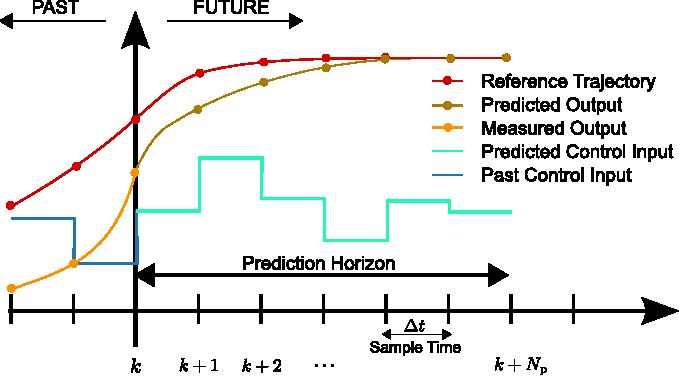
\includegraphics[height=0.4\textheight]{fig/lec01/MPC.pdf}
\caption{MPC scheme (source: \href{https://de.wikipedia.org/wiki/Model_Predictive_Control}{www.wikipedia.org},  by Martin Behrendt \href{https://creativecommons.org/licenses/by-sa/3.0/deed.en}{CC BY-SA 3.0})}
\end{figure}
}

%%%%%%%%%%%%%%%%%%%%%%%%%%%%%%%%%%%%%%%%%%%%%%%%%%%%%%%%%%%%%
%% Application examples with safety concerns %%
%%%%%%%%%%%%%%%%%%%%%%%%%%%%%%%%%%%%%%%%%%%%%%%%%%%%%%%%%%%%%
\frame{\frametitle{Application examples with safety-relevant constraints}
\begin{figure}
 \centering
 \begin{columns}
        \column{.2\linewidth}
				\caption*{Collaborative robot control (source: \href{https://commons.wikimedia.org/wiki/File:Human-Robot-Collaboration-Sawing-2016-Luka-Peternel.jpg}{www.wikipedia.org}, \href{https://creativecommons.org/licenses/by-sa/4.0/deed.en}{CC BY-SA 4.0})}
        \column{.3\linewidth}
        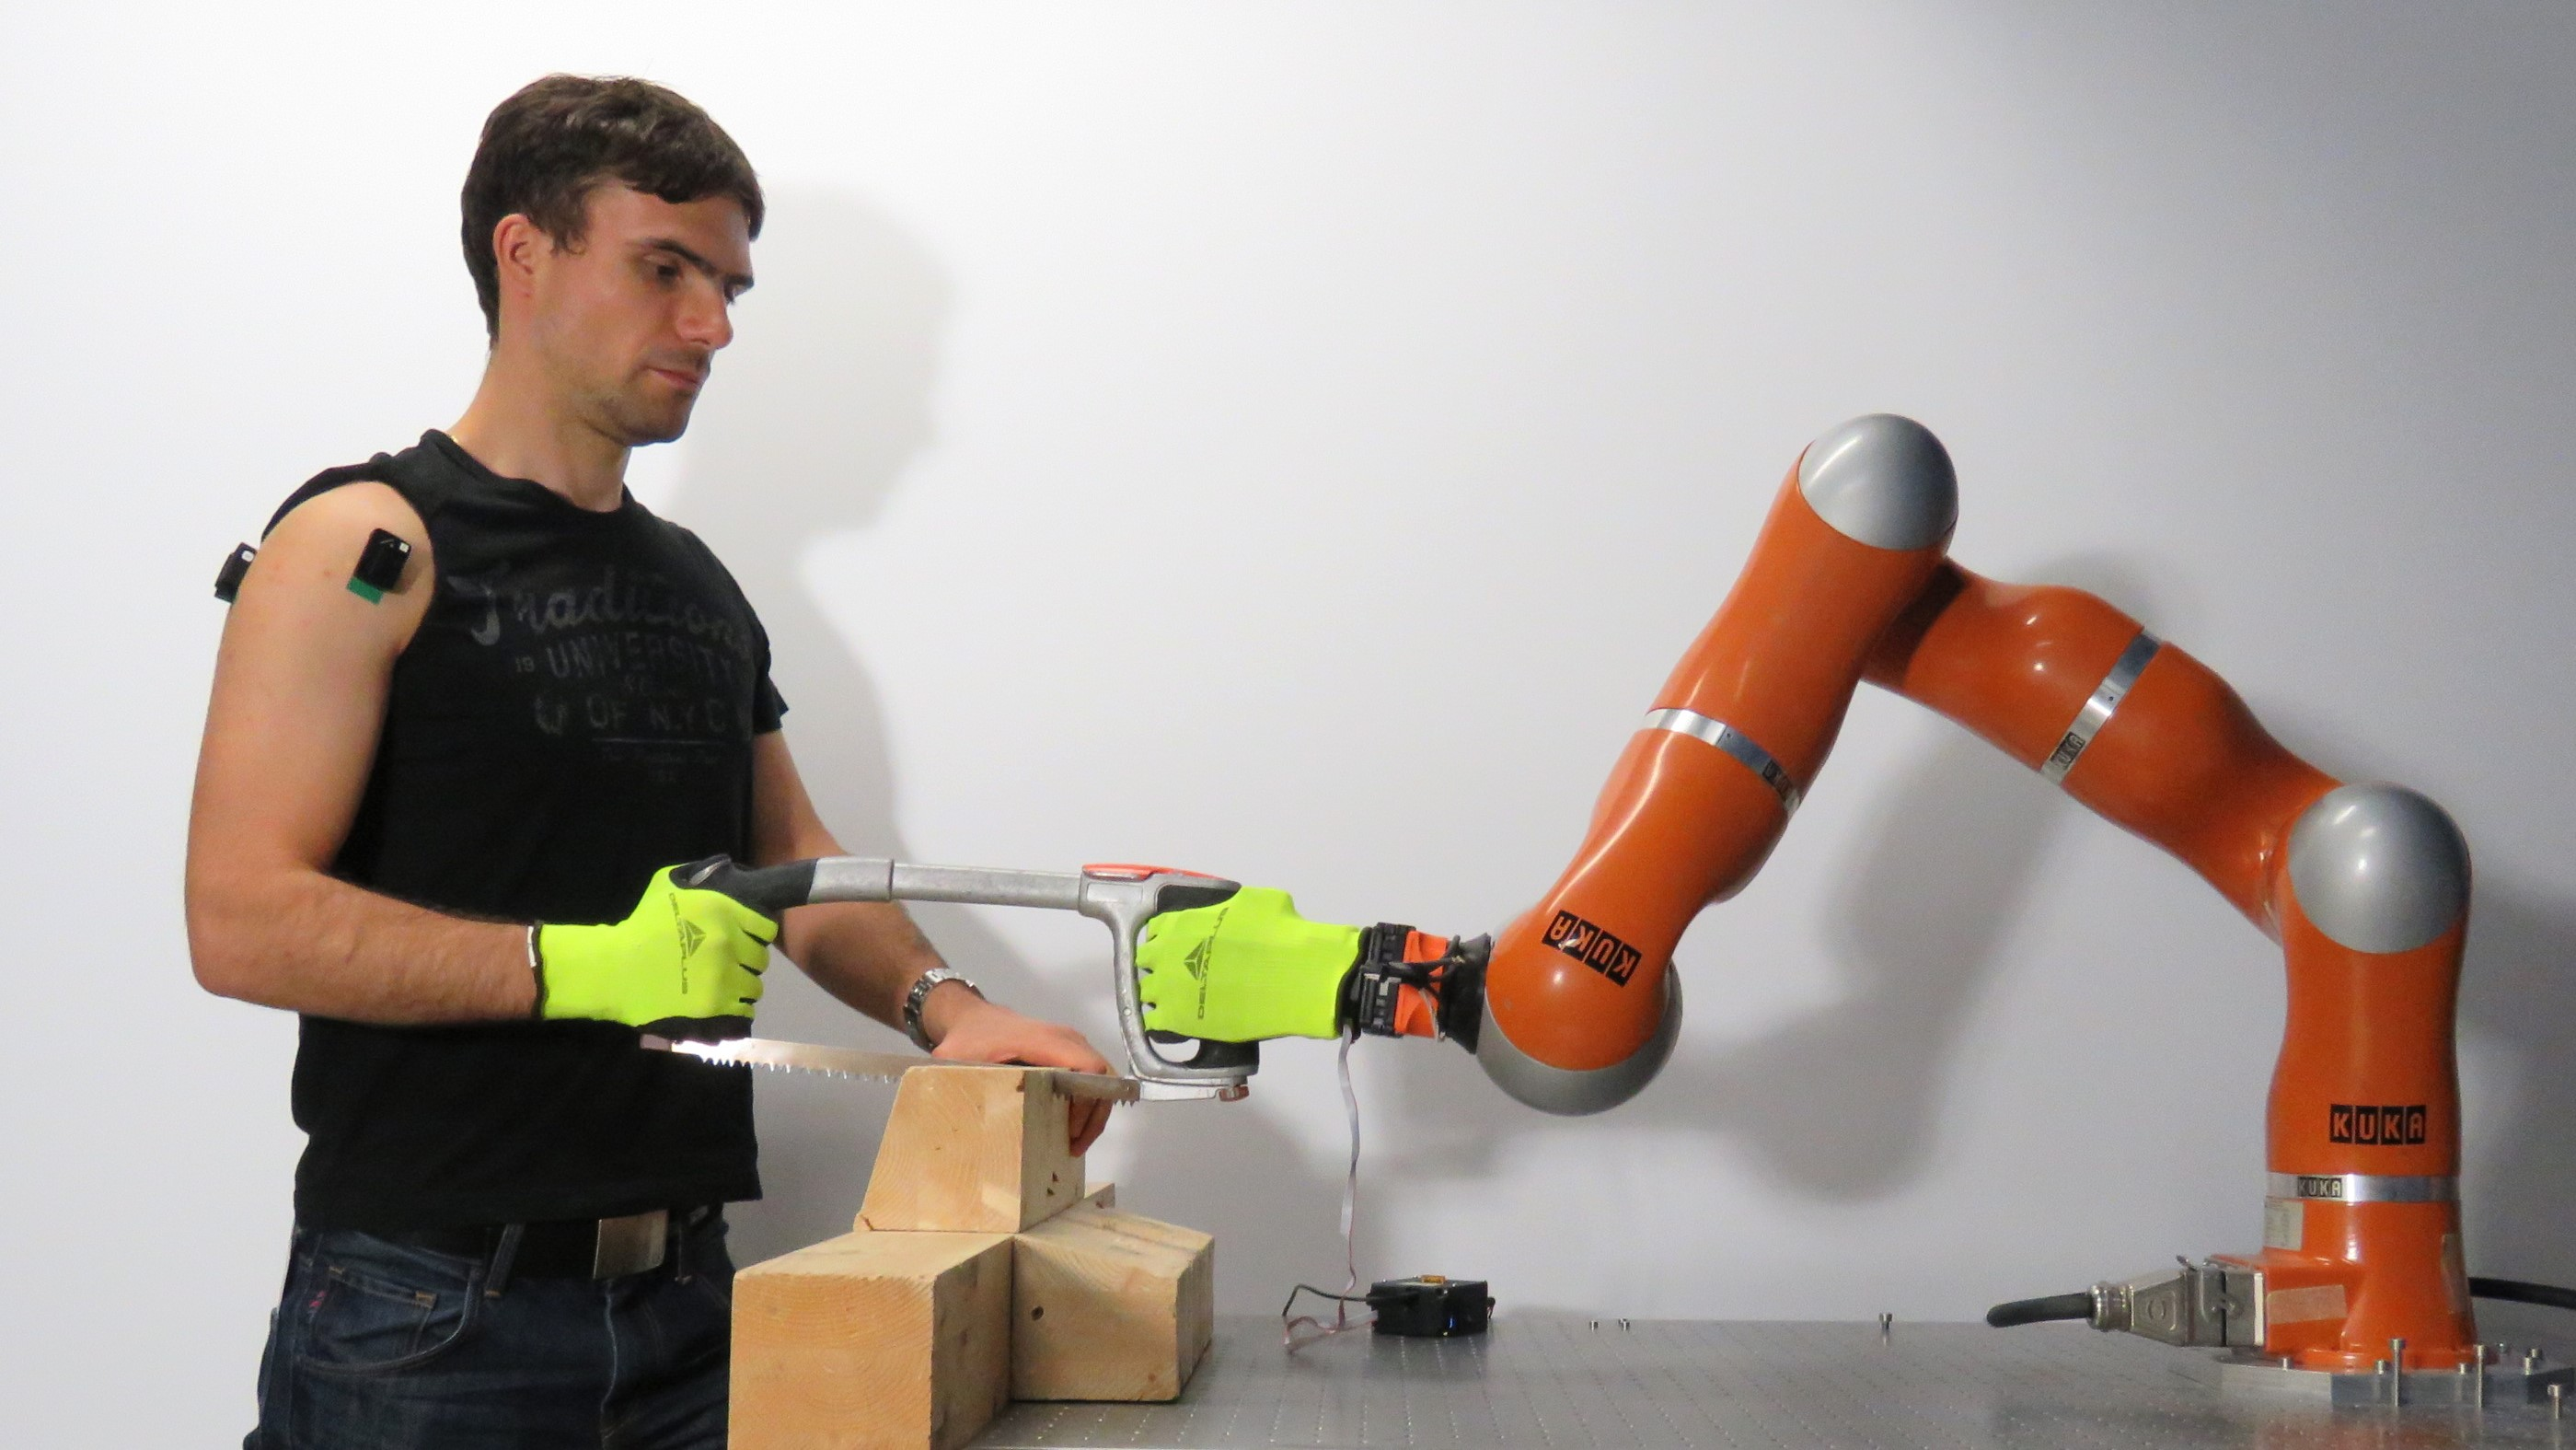
\includegraphics[width=\textwidth]{fig/lec14/Human-Robot-Collaboration.jpg}
				\column{.3\linewidth}
        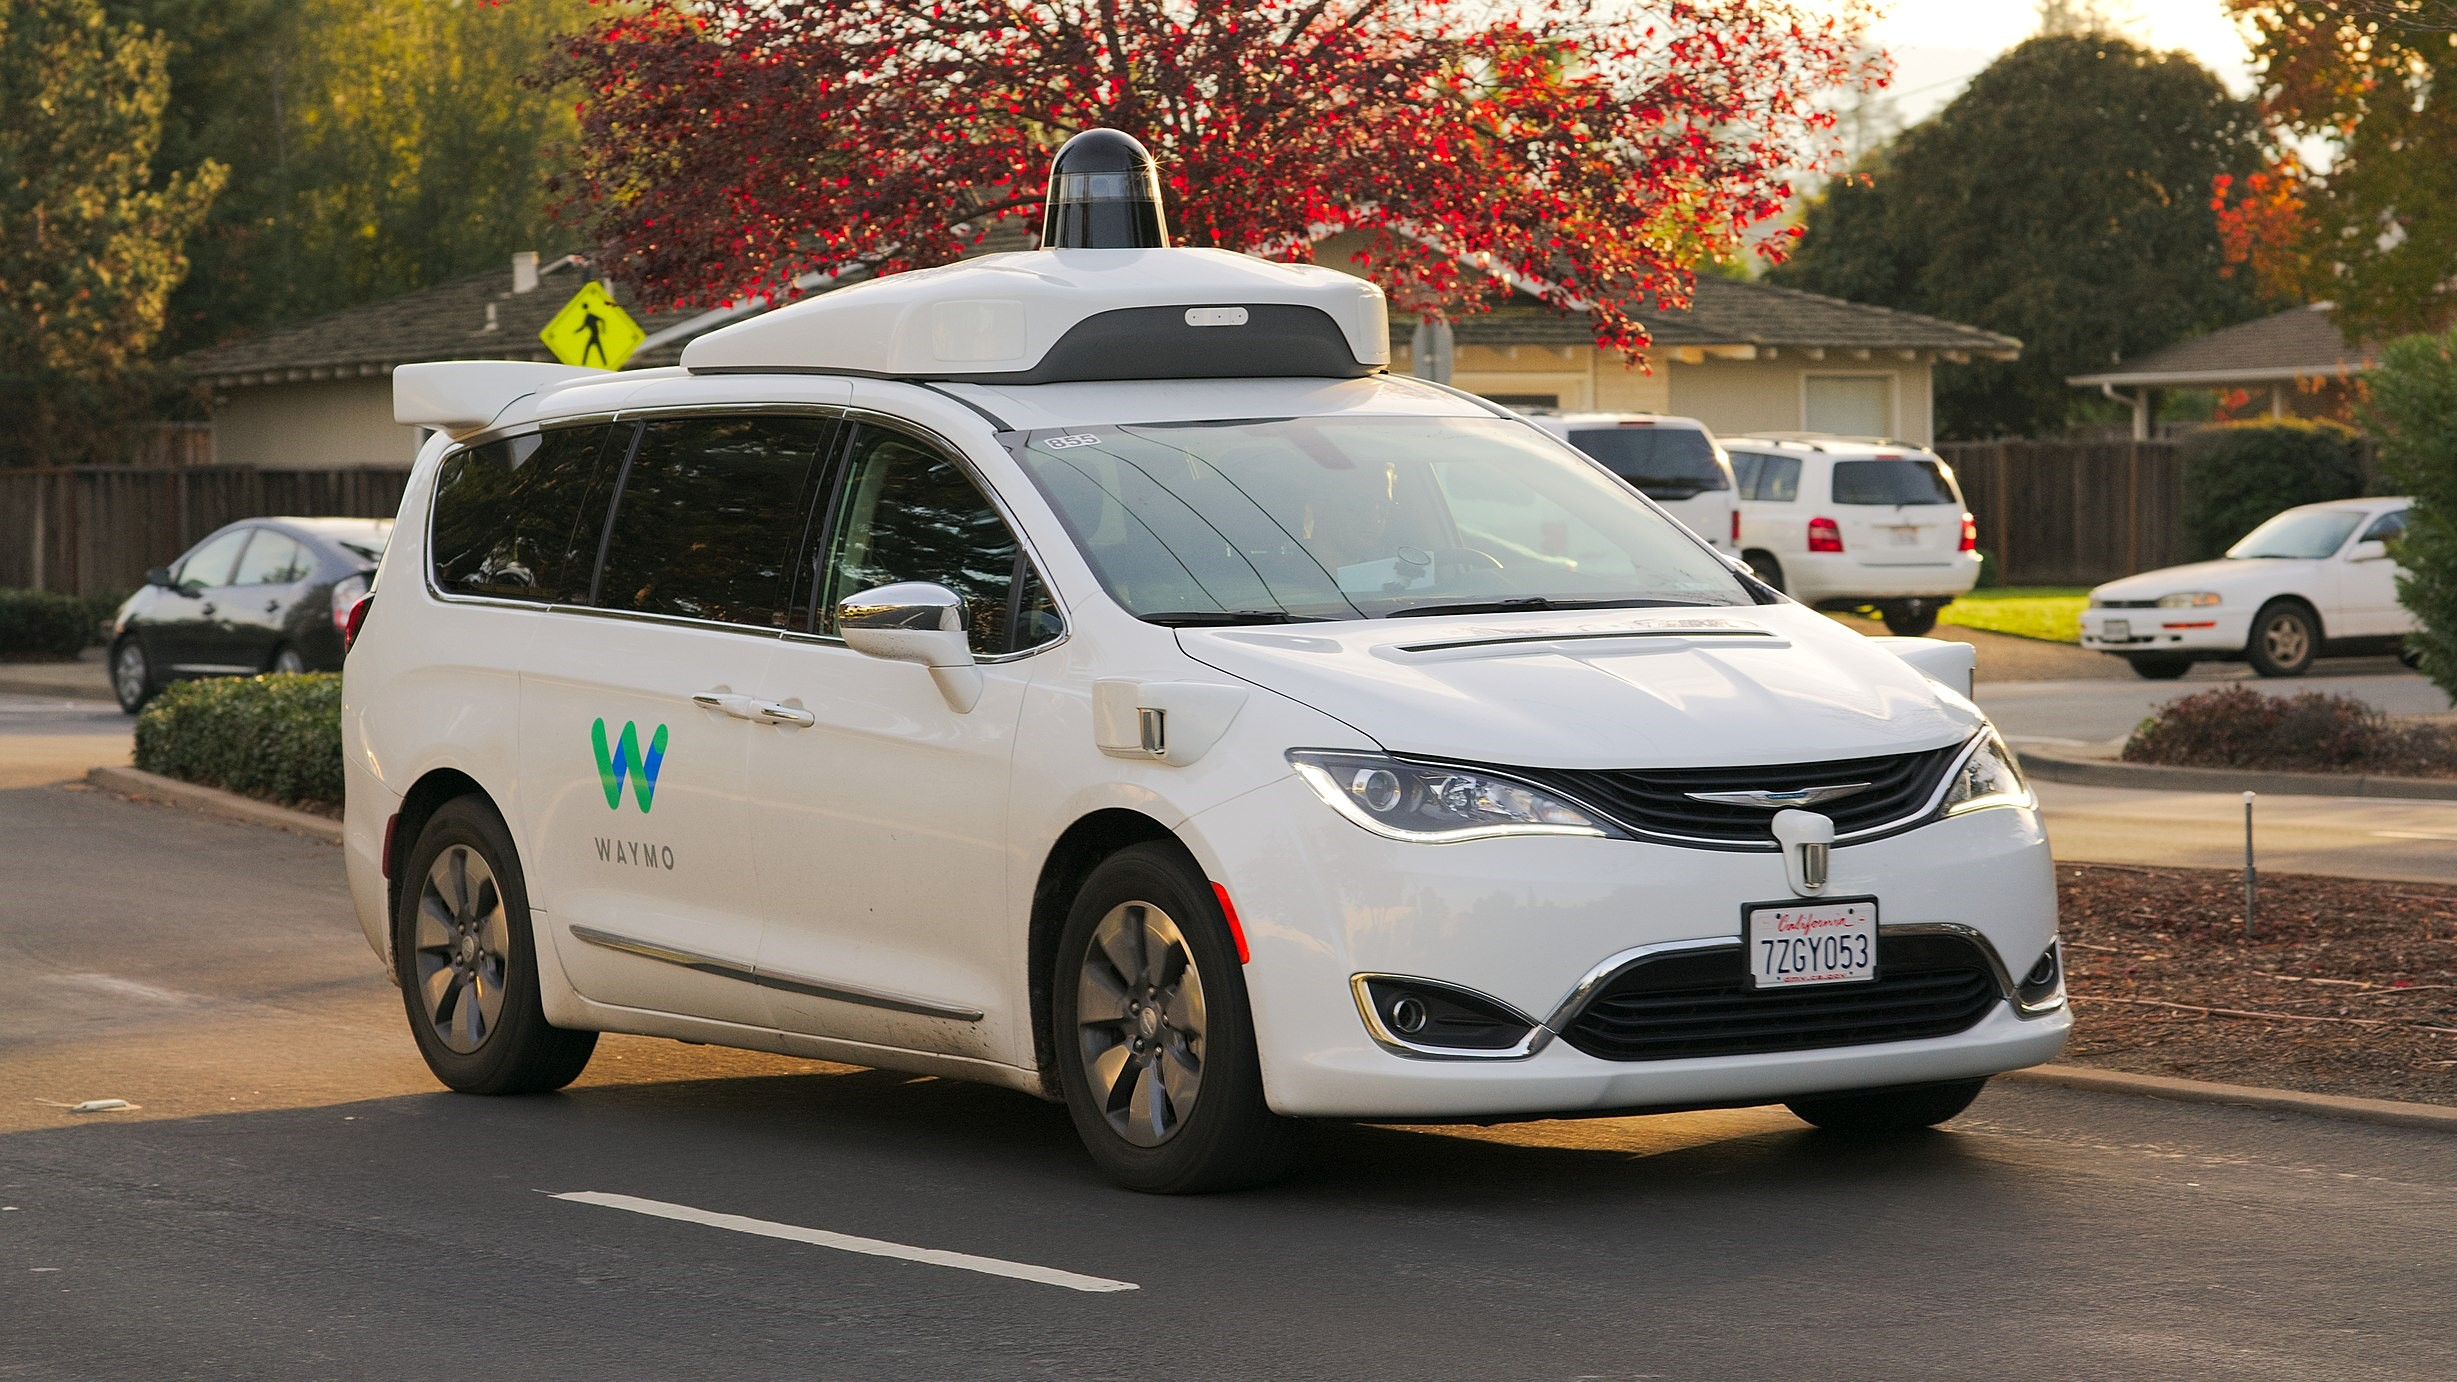
\includegraphics[width=\textwidth]{fig/lec14/Waymo.jpg}
				\column{.2\linewidth}
				\caption*{Autonomous car driving (source: \href{https://commons.wikimedia.org/wiki/File:Waymo_Chrysler_Pacifica_in_Los_Altos,_2017.jpg}{www.wikipedia.org}, \href{https://creativecommons.org/licenses/by-sa/4.0/deed.en}{CC BY-SA 4.0})}
      \end{columns}
			\vspace{1cm}
			\begin{columns}
        \column{.2\linewidth}
				\caption*{Energy system control}
        \column{.3\linewidth}
        \includegraphics[width=\textwidth]{fig/lec14/microgrid.jpg}
				\column{.3\linewidth}
        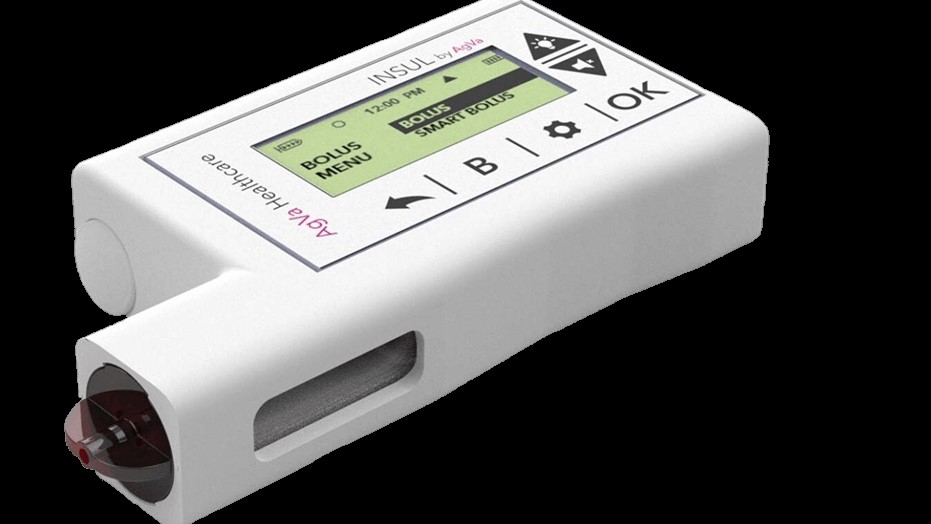
\includegraphics[width=\textwidth]{fig/lec14/Insulin_pump.jpg}
				\column{.2\linewidth}
				\caption*{Medication control (source: \href{https://commons.wikimedia.org/wiki/File:Insulin_pump.png}{www.wikipedia.org}, \href{https://creativecommons.org/licenses/by-sa/4.0/deed.en}{CC BY-SA 4.0})}
      \end{columns}
    \end{figure}
}

%%%%%%%%%%%%%%%%%%%%%%%%%%%%%%%%%%%%%%%%%%%%%%%%%%%%%%%%%%%%%
%% Safety levels %%
%%%%%%%%%%%%%%%%%%%%%%%%%%%%%%%%%%%%%%%%%%%%%%%%%%%%%%%%%%%%%
\frame{\frametitle{Safety levels}
\begin{figure}
\centering
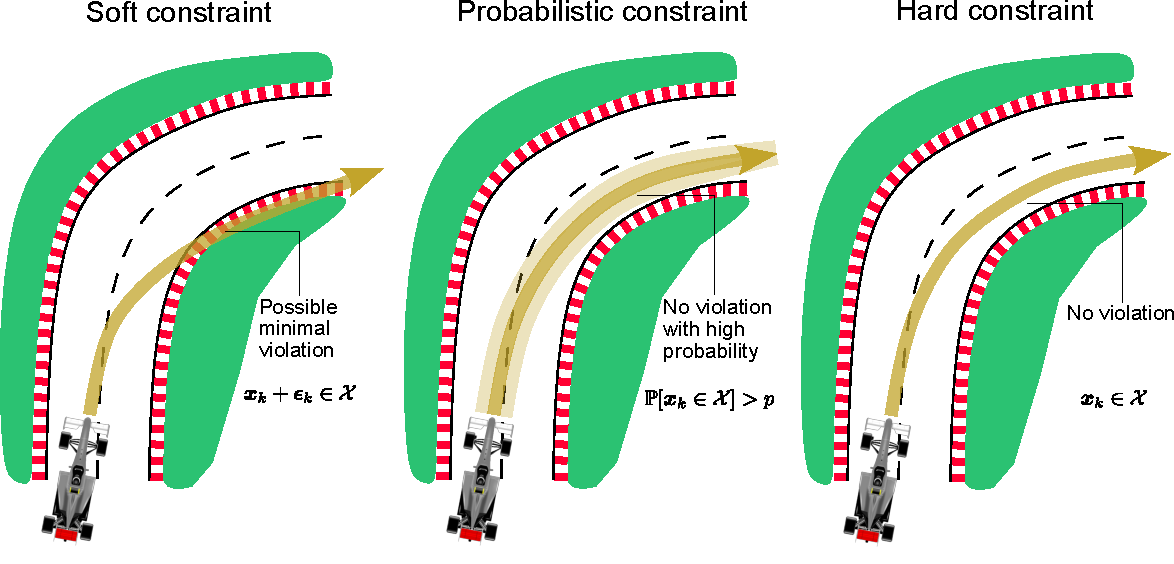
\includegraphics[height=0.68\textheight]{fig/lec14/Safety_Levels.pdf}
\caption{Different levels of safety (derived from L. Brunke et al., \textit{Safe Learning in Robotics: From Learning-Based Control to Safe Reinforcement Learning}, Annual Review of Control, Robotics, and Autonomous Systems, 2022)}
\label{fig:safety_levels}
\end{figure}
}

%%%%%%%%%%%%%%%%%%%%%%%%%%%%%%%%%%%%%%%%%%%%%%%%%%%%%%%%%%%%%
%% Bird's eye view on RL concepts integrating safety %%
%%%%%%%%%%%%%%%%%%%%%%%%%%%%%%%%%%%%%%%%%%%%%%%%%%%%%%%%%%%%%
\frame{\frametitle{Bird's eye view on RL concepts integrating safety}
\vspace{-0.1cm}
\begin{figure}%
\centering
\subfloat[][Safety critic: add a critic which indicates to which extent the current data sample fits to a safe situation]{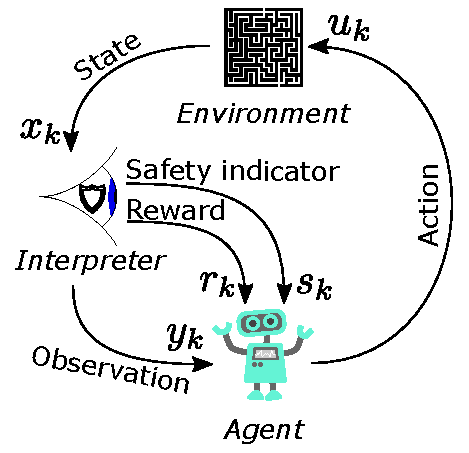
\includegraphics[width=0.375\textwidth]{fig/lec14/RL_Safety_Critic.pdf}}%
\qquad
\subfloat[][Safety shield: use a priori or learned model knowledge of the environment to make predictions identifying actions leading to unsafe situations]{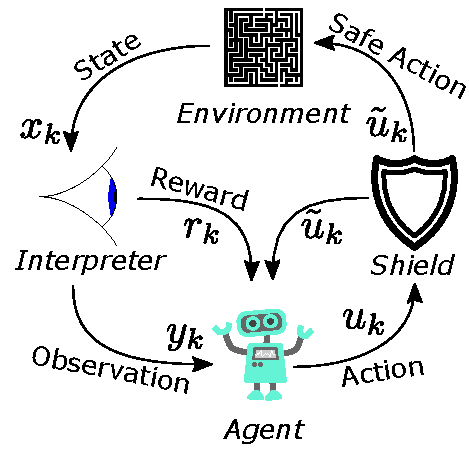
\includegraphics[width=0.375\textwidth]{fig/lec14/Safe_RL_Shield.pdf}}%
\label{fig:safety_birds_eye}%
\end{figure}
}

%%%%%%%%%%%%%%%%%%%%%%%%%%%%%%%%%%%%%%%%%%%%%%%%%%%%%%%%%%%%%
%% Bird's eye view on RL concepts integrating safety %%
%%%%%%%%%%%%%%%%%%%%%%%%%%%%%%%%%%%%%%%%%%%%%%%%%%%%%%%%%%%%%
\frame{\frametitle{Achievable safety levels and model knowledge}
\begin{figure}
\centering
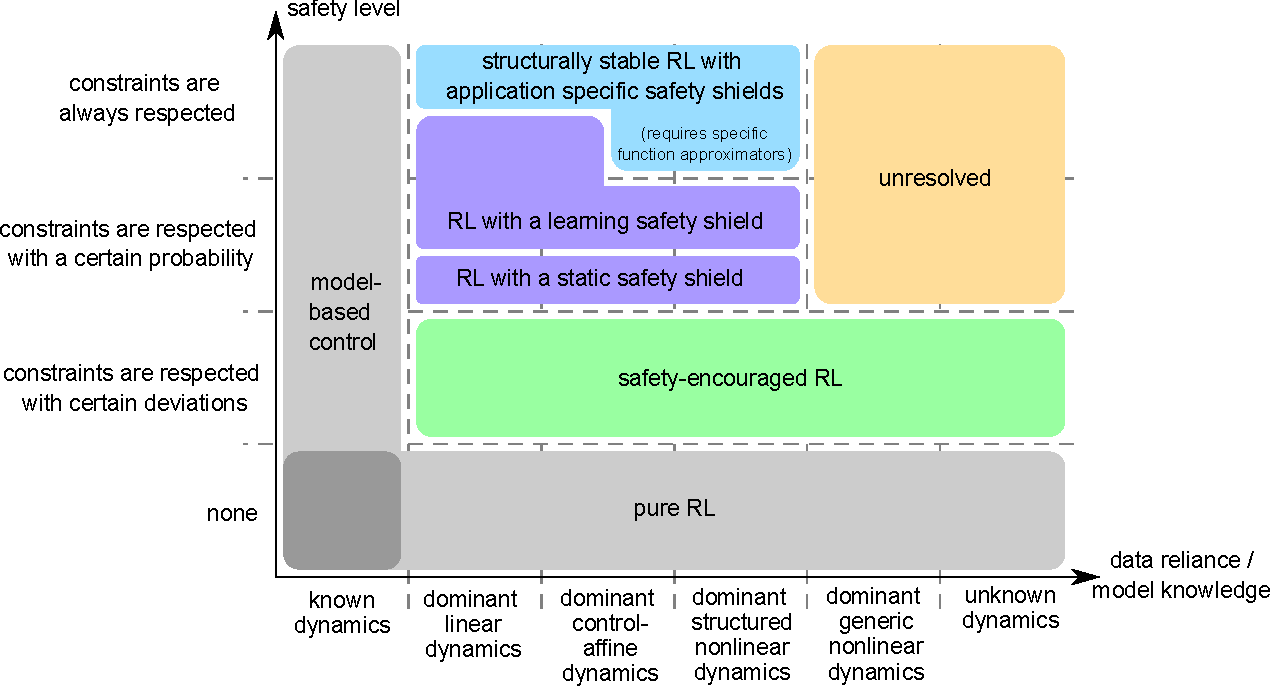
\includegraphics[height=0.68\textheight]{fig/lec14/Safeguard_Classes.pdf}
\caption{Safety and model knowledge map (derived from L. Brunke et al., \textit{Safe Learning in Robotics: From Learning-Based Control to Safe Reinforcement Learning}, Annual Review of Control, Robotics, and Autonomous Systems, 2022)}
\end{figure}
}

%%%%%%%%%%%%%%%%%%%%%%%%%%%%%%%%%%%%%%%%%%%%%%%%%%%%%%%%%%%%%
%% MG Safe application %%
%%%%%%%%%%%%%%%%%%%%%%%%%%%%%%%%%%%%%%%%%%%%%%%%%%%%%%%%%%%%%
\frame{\frametitle{Energy system control application}
\vspace{-0.1cm}
\begin{figure}%
\centering
\subfloat[][Example microgrid that can be emulated in the \href{https://ei.uni-paderborn.de/lea/research/forschungsprojekte/intelligent-energy-systems/microgrid-laboratory}{LEA Microgrid Laboratory}.]{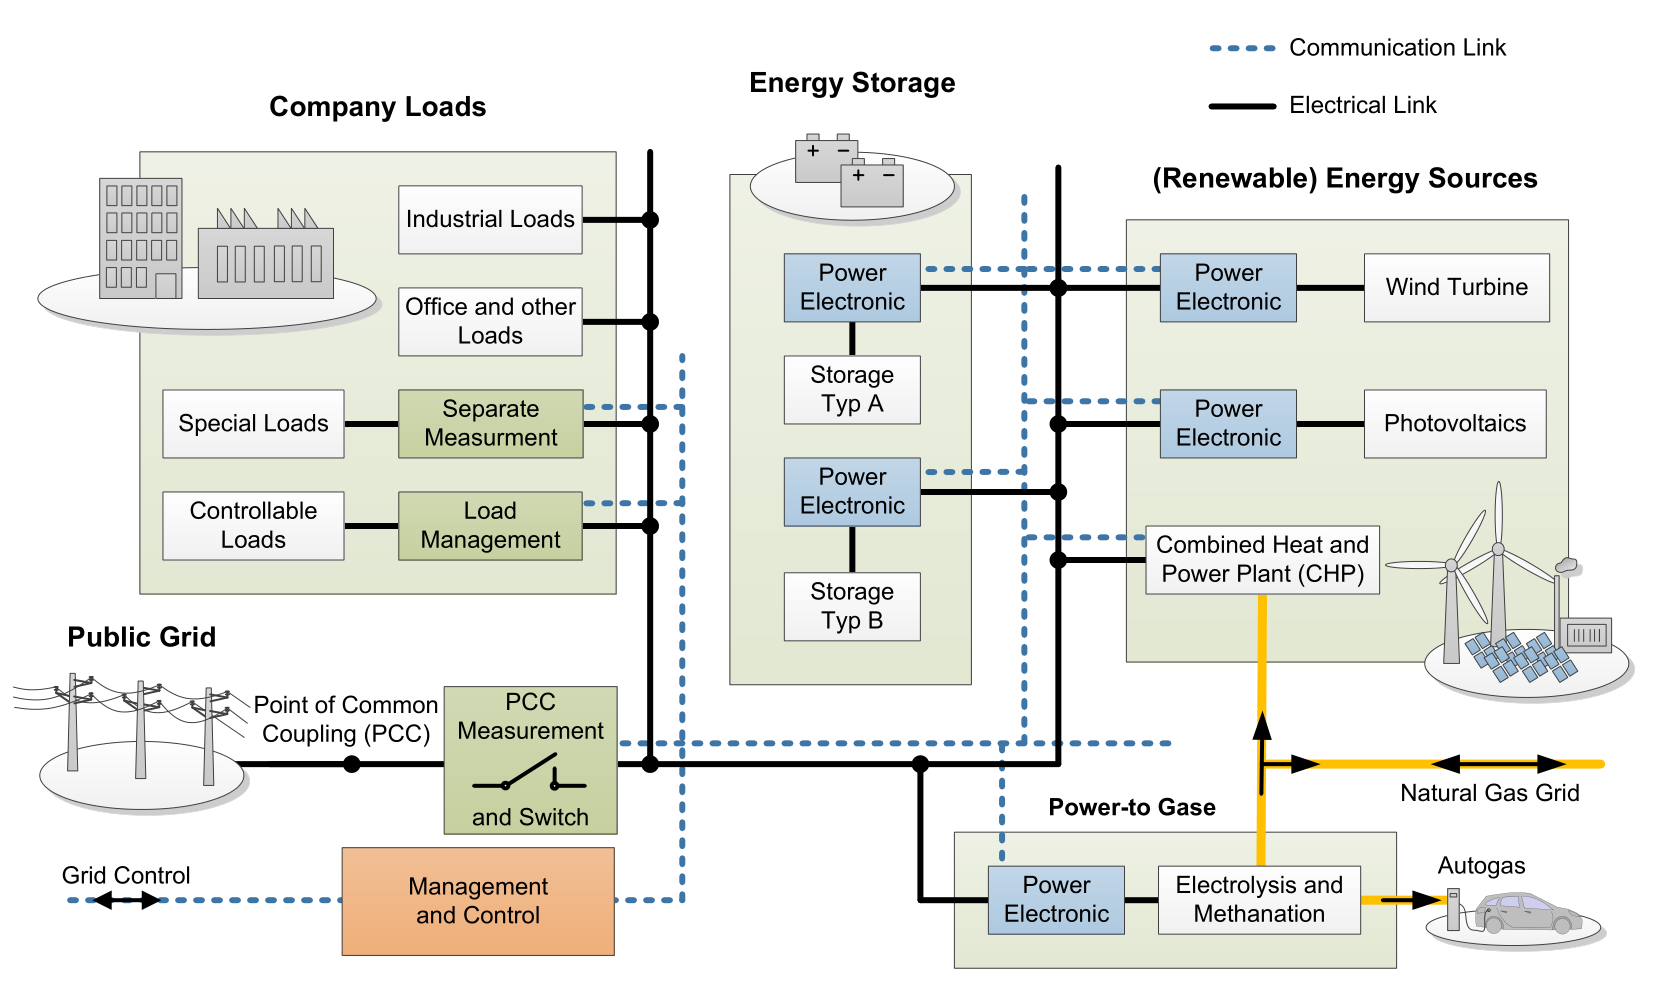
\includegraphics[width=0.45\textwidth]{fig/lec14/MG_vogt.png}}%
\qquad
\subfloat[][Application under investigation: Three-phase grid-forming inverter disturbed by stochastic load]{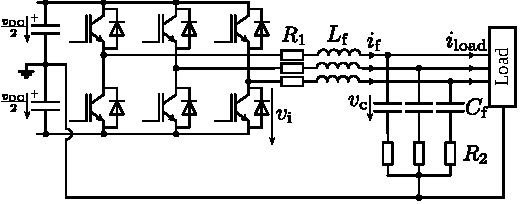
\includegraphics[width=0.45\textwidth]{fig/lec14/UPS_LC_Structure.pdf}}%
\label{fig:MG_application}%
\end{figure}
}


%%%%%%%%%%%%%%%%%%%%%%%%%%%%%%%%%%%%%%%%%%%%%%%%%%%%%%%%%%%%%
%% OMG + system constraints%%
%%%%%%%%%%%%%%%%%%%%%%%%%%%%%%%%%%%%%%%%%%%%%%%%%%%%%%%%%%%%%
\frame{\frametitle{Reference tracking with disturbance rejection}
\begin{columns}[t,onlytextwidth]
\begin{column}{0.475\textwidth}
\begin{minipage}[c]{\linewidth}
\begin{figure}
	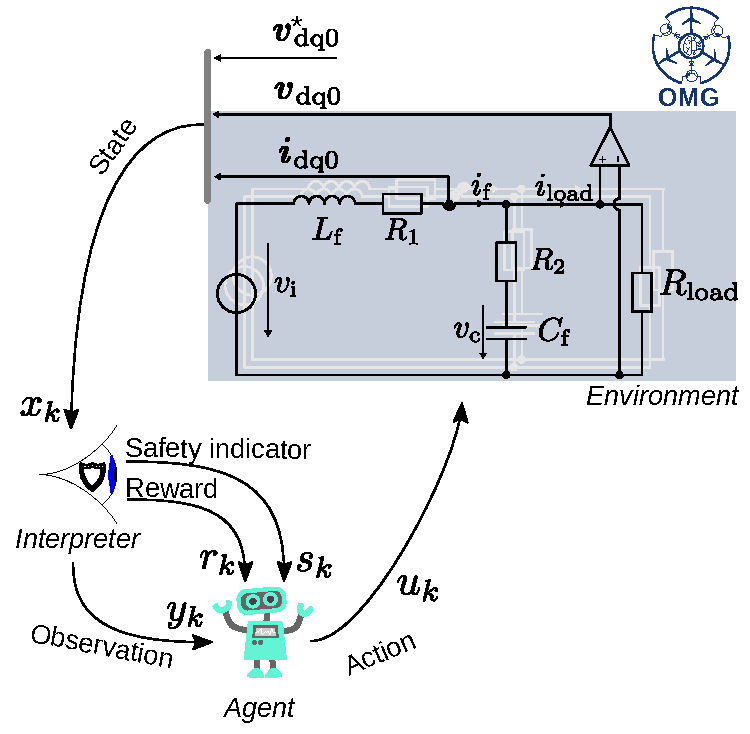
\includegraphics[width=0.8\textwidth, height=0.65\textheight]{fig/lec14/RL_Safety_Critic_OMG.pdf}
	\caption{Simulation setting with environment modeled using \href{https://github.com/upb-lea/openmodelica-microgrid-gym}{OpenModelica Microgrid Gym}}
	\label{fig:RL_OMG}
\end{figure}
\end{minipage}
\end{column}
\hfill
\begin{column}{0.54\textwidth}
\begin{minipage}[c]{\linewidth}
\begin{itemize}
	\item Cont. state- and actionspace
	\item Deep deterministic policy gradient agent
	\item Gird-forming inverter
	\item Stochastic load acts as disturbance
	\item State per phase: $\bm{x_k} = [i_\mathrm{f}, v_\mathrm{C_\mathrm{}}]$, $v_\mathrm{i} = v_\mathrm{DC} \cdot u_{k\mathrm{}}$
	\item $r_k=f(v_\mathrm{C}, v^*, i_\mathrm{f}) \in [1, -0.75]$
	%, i.e., goal is to supply load with voltage $v^*$
	\item $s_k = -1$, if limit ($i_\mathrm{f} \text{ or } v_\mathrm{C_\mathrm{}}$) is exceeded
\end{itemize}
\end{minipage}
\end{column}
\end{columns}
}

%%%%%%%%%%%%%%%%%%%%%%%%%%%%%%%%%%%%%%%%%%%%%%%%%%%%%%%%%%%%%
%% Reward function grid application
%%%%%%%%%%%%%%%%%%%%%%%%%%%%%%%%%%%%%%%%%%%%%%%%%%%%%%%%%%%%%
\frame{\frametitle{Reward design for grid-forming inverter}
\begin{columns}[t,onlytextwidth]
\begin{column}{0.475\textwidth}
\begin{minipage}[c]{\linewidth}
\begin{figure}
	%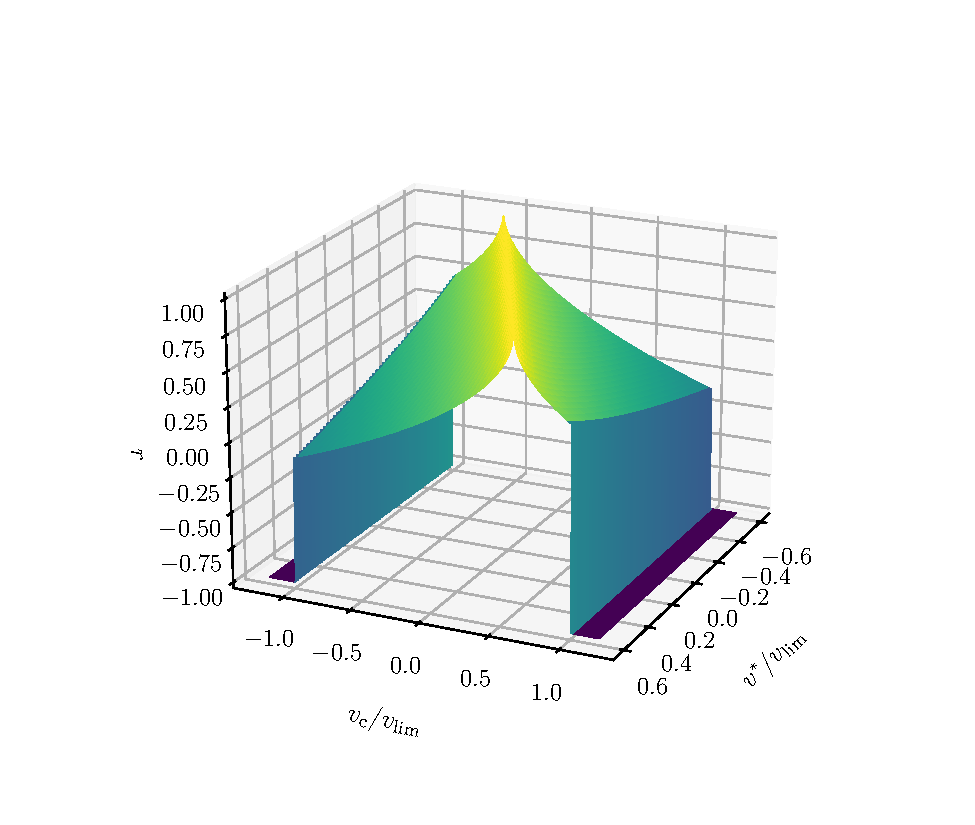
\includegraphics[width=1.11\textwidth, height=0.8\textheight]{fig/lec14/Reward_v_mre.pdf}
	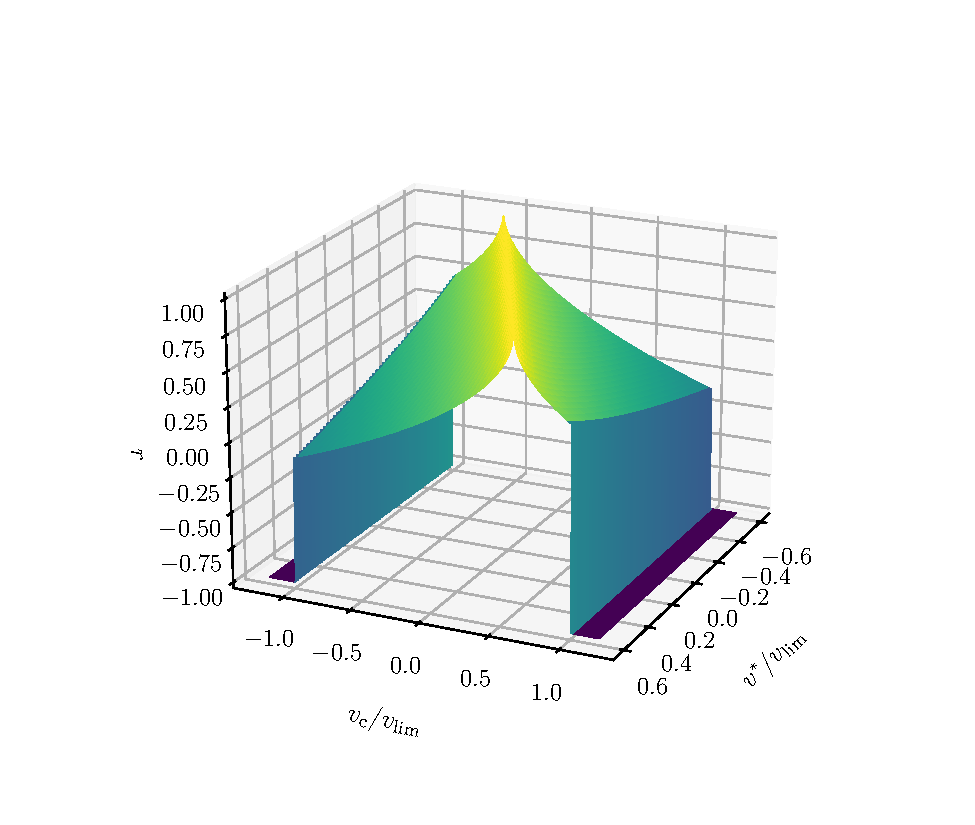
\includegraphics[trim=50 40 10 60, clip, width=1.1\linewidth]{fig/lec14/Reward_v_mre.pdf}
	\caption{Reward function \ref{eq:reward} for different reference and measured voltages and currents below nominal current}
\end{figure}
\end{minipage}
\end{column}
\hfill
\begin{column}{0.54\textwidth}
\begin{minipage}[c]{\linewidth}
\begin{itemize}
	\item Three cases, depending on operation point
\end{itemize}
\begin{align}
    r_{} =
    \begin{cases}
         \text{MRE}(v_\mathrm{C}, v^*) , &
         \Large\textcircled{\raisebox{.4pt}{\normalsize\textbf A}} \\
         %
         \text{MRE}(v_\mathrm{C}, v^*) + f(i_\mathrm{f}), & \Large\textcircled{\raisebox{.4pt}{\normalsize\textbf B}} \\
         %
         -1, & \Large\textcircled{\raisebox{.4pt}{\normalsize\textbf C}}
    \end{cases}
    \label{eq:reward}
\end{align}
\begin{itemize}
	\item \Large\textcircled{\raisebox{.4pt}{\normalsize\textbf A}} $v_{\text{C}} \leq v_\mathrm{lim} \, \wedge\,  i_{\text{f}} \leq i_\mathrm{nom}$
	\item \Large\textcircled{\raisebox{.4pt}{\normalsize\textbf B}} $v_{\text{C}} \leq v_\mathrm{lim} \, \wedge\, i_\mathrm{nom} \leq i_{\text{f}} \leq i_\mathrm{lim}$
	\item \Large\textcircled{\raisebox{.4pt}{\normalsize\textbf C}} otherwise
	\item Linear punishment term $f(i_\mathrm{f})$
	%\item
\end{itemize}
\end{minipage}
\end{column}
\end{columns}
}

%%%%%%%%%%%%%%%%%%%%%%%%%%%%%%%%%%%%%%%%%%%%%%%%%%%%%%%%%%%%%
%% OMG + safeguard%%
%%%%%%%%%%%%%%%%%%%%%%%%%%%%%%%%%%%%%%%%%%%%%%%%%%%%%%%%%%%%%
\frame{\frametitle{Reference tracking with disturbance rejection using saftey shield}
\begin{columns}[t,onlytextwidth]
\begin{column}{0.475\textwidth}
\begin{minipage}[c]{\linewidth}
\begin{figure}
	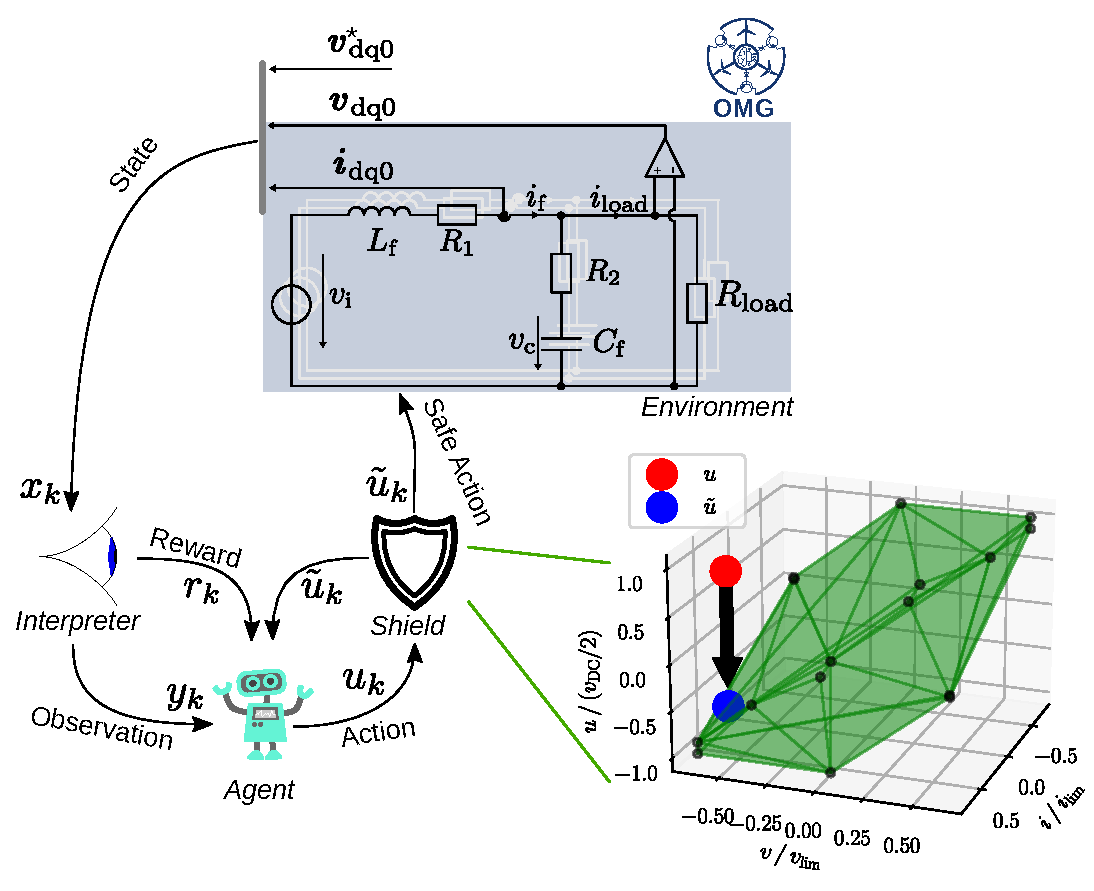
\includegraphics[width=0.9\textwidth, height=0.65\textheight]{fig/lec14/Safe_RL_Shield_OMG.pdf}
	\caption{Safety shield based on feasible set}
\end{figure}
\end{minipage}
\end{column}
\hfill
\begin{column}{0.54\textwidth}
\begin{minipage}[c]{\linewidth}
\begin{itemize}
	\item Safety shield: Ensure that action does not cause state limit violation in future system trajectories
	\item Such a state action pair is called feasible
	\item Calculation of \textcolor{signalgreen}{feasible set} requires a model
	\item Training data can be utilized to \href{https://ei.uni-paderborn.de/en/lea/teaching/veranstaltungen/teaching/translate-to-english-systemidentifikation}{identify} model
	\item Here, recursive least squares (RLS) is applied
\end{itemize}
\end{minipage}
\end{column}
\end{columns}
}

%%%%%%%%%%%%%%%%%%%%%%%%%%%%%%%%%%%%%%%%%%%%%%%%%%%%%%%%%%%%%
%% OMG + safeguard results%%
%%%%%%%%%%%%%%%%%%%%%%%%%%%%%%%%%%%%%%%%%%%%%%%%%%%%%%%%%%%%%
\frame{\frametitle{Saftey shield based on feasible set - proof of concept (1)}
\begin{columns}[t,onlytextwidth]
\begin{column}{0.475\textwidth}
\begin{minipage}[c]{\linewidth}
\begin{figure}
	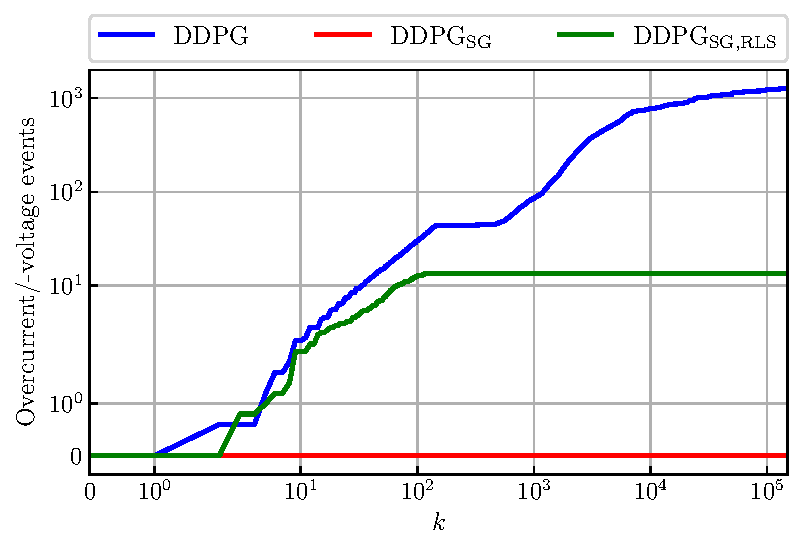
\includegraphics[width=0.85\textwidth, height=0.55\textheight]{fig/lec14/OMG_all_aborts_log.pdf}
	\caption{Accumulated unsafe events (overcurrent/-voltage) per training step $k$}
\end{figure}
\end{minipage}
\end{column}
\hfill
\begin{column}{0.54\textwidth}
\begin{minipage}[c]{\linewidth}
\begin{itemize}
	\item Three different approaches
	\item \textcolor{signalblue}{$\mathrm{DDPG}_\mathrm{}$}: Agent without safety shield
	\item \textcolor{signalred}{$\mathrm{DDPG}_\mathrm{SG}$}: Agent with safety shield using perfect a priori knowledge
	\item \textcolor{signalgreen}{$\mathrm{DDPG}_\mathrm{SG,RLS}$}: Agent with safety shield without a priori knowledge, identifying model using RLS
	\item Five agents trained per approach
	\item Results in D. Weber et al., \textit{Safe Reinforcement Learning-Based Control in
Power Electronic Systems}, 2023, doi: \href{https://ieeexplore.ieee.org/abstract/document/10182718}{10.1109/FES57669.2023.10182718}
\end{itemize}
\end{minipage}
\end{column}
\end{columns}
}

%%%%%%%%%%%%%%%%%%%%%%%%%%%%%%%%%%%%%%%%%%%%%%%%%%%%%%%%%%%%%
%% OMG + safeguard results%%
%%%%%%%%%%%%%%%%%%%%%%%%%%%%%%%%%%%%%%%%%%%%%%%%%%%%%%%%%%%%%
\frame{\frametitle{Saftey shield based on feasible set - proof of concept (2)}
\begin{columns}[t,onlytextwidth]
\begin{column}{0.54\textwidth}
\begin{minipage}[c]{\linewidth}
	\vspace{0.25cm}
\begin{figure}
	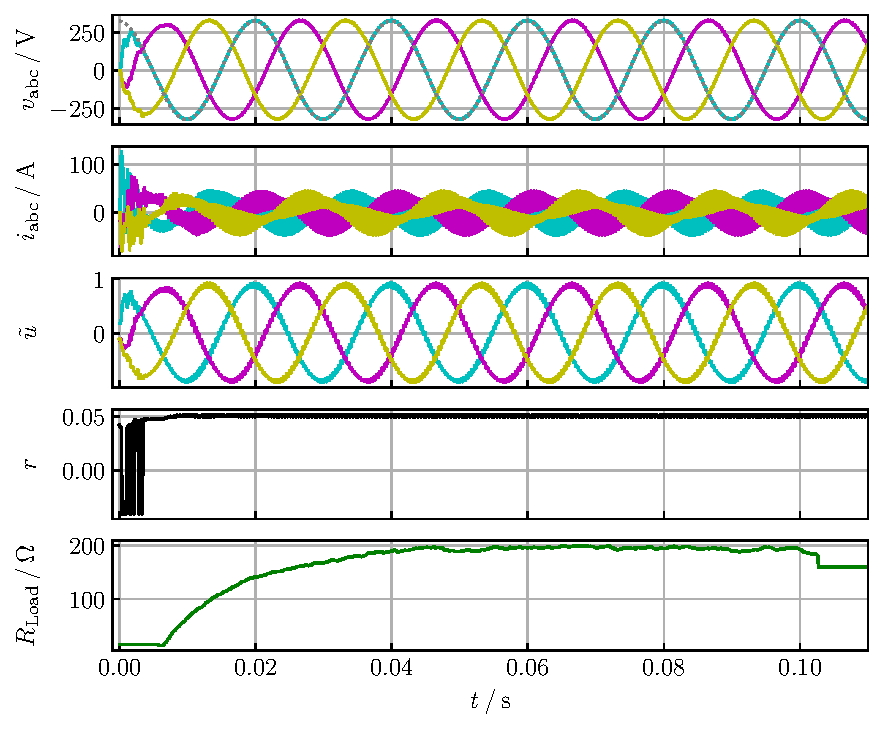
\includegraphics[width=0.9\textwidth]{fig/lec14/370_vDC_SL_RLS_varLoadtimeseries_testcase.pdf}
	\caption{Blackstart after training using \textcolor{signalgreen}{$\mathrm{DDPG}_\mathrm{SG,RLS}$}}
\end{figure}
\end{minipage}
\end{column}
\hfill
\begin{column}{0.45\textwidth}
\begin{minipage}[c]{\linewidth}
\begin{itemize}
	\item $\mathrm{DDPG}_\mathrm{SG,RLS}$ agent trained for 150000 steps
	\item $R_\mathrm{Load}$ changes every step based on random process
	\item Additional events -- load steps and drifts -- triggered randomly
\end{itemize}
\end{minipage}
\end{column}
\end{columns}
}

%%%%%%%%%%%%%%%%%%%%%%%%%%%%%%%%%%%%%%%%%%%%%%%%%%%%%%%%%%%%%%%%%%
\subsection{Real-world implementation with fast policy inference} 
%%%%%%%%%%%%%%%%%%%%%%%%%%%%%%%%%%%%%%%%%%%%%%%%%%%%%%%%%%%%%%%%%%


%%%%%%%%%%%%%%%%%%%%%%%%%%%%%%%%%%%%%%%%%%%%%%%%%%%%%%%%%%%%%
%% Real-time implementation aspects %%
%%%%%%%%%%%%%%%%%%%%%%%%%%%%%%%%%%%%%%%%%%%%%%%%%%%%%%%%%%%%%
\frame{\frametitle{Real-time implementation aspects (1)}
\begin{figure}
\centering
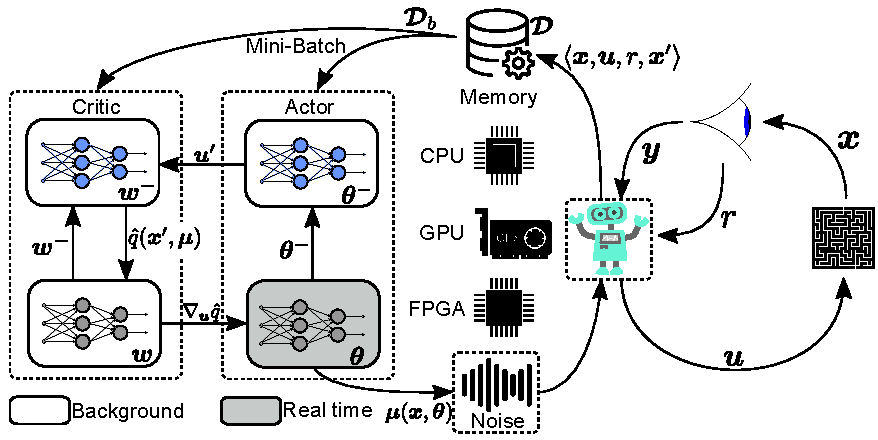
\includegraphics[height=0.68\textheight]{fig/lec14/DDPG_Real_Time.pdf}
\caption{DDPG implementation example (derivative work of \figref{fig:RL_Wiki} and \href{https://commons.wikimedia.org/wiki/File:Multi-Layer_Neural_Network-Vector.svg?uselang=de}{wikipedia.org}, \href{https://creativecommons.org/publicdomain/zero/1.0/deed.en}{CC0 1.0})}
\label{fig:DDPG_Real_Time}
\end{figure}
}

%%%%%%%%%%%%%%%%%%%%%%%%%%%%%%%%%%%%%%%%%%%%%%%%%%%%%%%%%%%%%
%% Real-time implementation aspects 2 %%
%%%%%%%%%%%%%%%%%%%%%%%%%%%%%%%%%%%%%%%%%%%%%%%%%%%%%%%%%%%%%
\frame{\frametitle{Real-time implementation aspects (2)}
\vspace{-0.1cm}
\begin{figure}%
\centering
\subfloat[][Real-time control requirement vs. learning time]{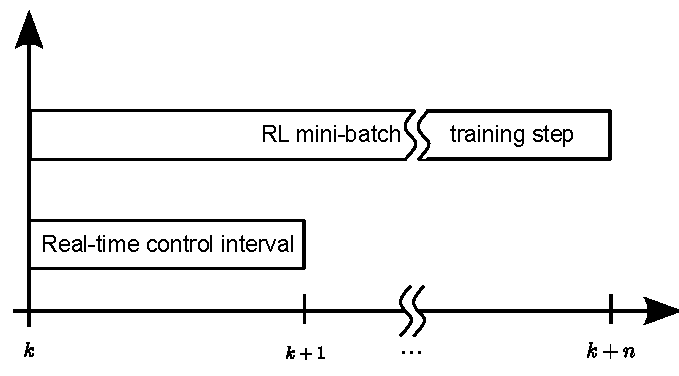
\includegraphics[width=0.45\textwidth]{fig/lec14/Timing.pdf}}%
\qquad
\subfloat[][Typical evolution of RL parameter weights during learning]{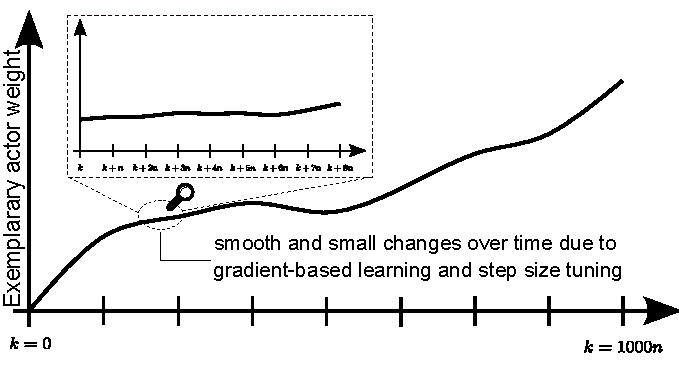
\includegraphics[width=0.45\textwidth]{fig/lec14/NN-Weights.pdf}}%
\label{fig:timing}%
\end{figure}
}

%%%%%%%%%%%%%%%%%%%%%%%%%%%%%%%%%%%%%%%%%%%%%%%%%%%%%%%%%%%%%
%% Control Scheme of the DQ-DTC %%
%%%%%%%%%%%%%%%%%%%%%%%%%%%%%%%%%%%%%%%%%%%%%%%%%%%%%%%%%%%%%
\frame{\frametitle{Application example: deep Q direct torque control}
\begin{columns}[t,onlytextwidth]
\begin{column}{0.54\textwidth}
\begin{minipage}[c]{\linewidth}
\begin{figure}
	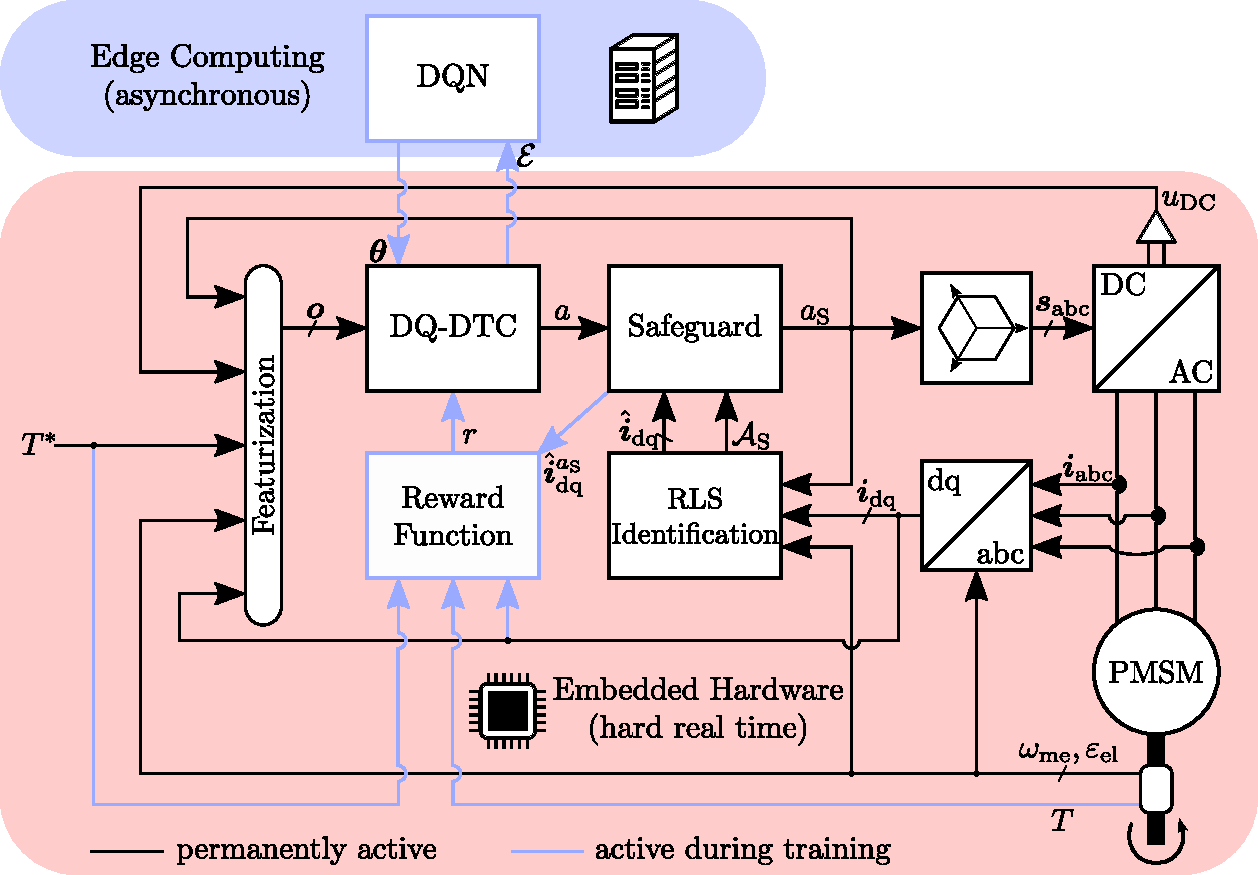
\includegraphics[scale=0.35]{fig/lec14/Safeguarded_DQDTC_Scheme.pdf}
	\caption{Deep Q direct torque control schematic}
	\label{fig:DQDTC_Scheme}
\end{figure}
\end{minipage}
\end{column}
\hfill
\begin{column}{0.45\textwidth}
\begin{minipage}[c]{\linewidth}
\begin{itemize}
	\item The DQ-DTC is basically a DQN
	\item Sampling time of the plant system is $T_\text{s}=\SI{50}{\micro\second}$
	\item DQN inference, safeguarding and system identification must fit into $T_\text{s}$
	\item Source: M. Schenke et al., \textit{Finite-Set Direct Torque Control via Edge Computing-Assisted
Safe Reinforcement Learning for a Permanent Magnet Synchronous Motor}, 2023, doi: \href{https://ieeexplore.ieee.org/abstract/document/10214121}{10.1109/TPEL.2023.3303651}
\end{itemize}
\end{minipage}
\end{column}
\end{columns}
}

%%%%%%%%%%%%%%%%%%%%%%%%%%%%%%%%%%%%%%%%%%%%%%%%%%%%%%%%%%%%%
%% Fast neural network inference %%
%%%%%%%%%%%%%%%%%%%%%%%%%%%%%%%%%%%%%%%%%%%%%%%%%%%%%%%%%%%%%
\frame{\frametitle{Fast neural network inference}
\begin{columns}[t,onlytextwidth]
\begin{column}{0.54\textwidth}
\begin{minipage}[c]{\linewidth}
\begin{figure}
	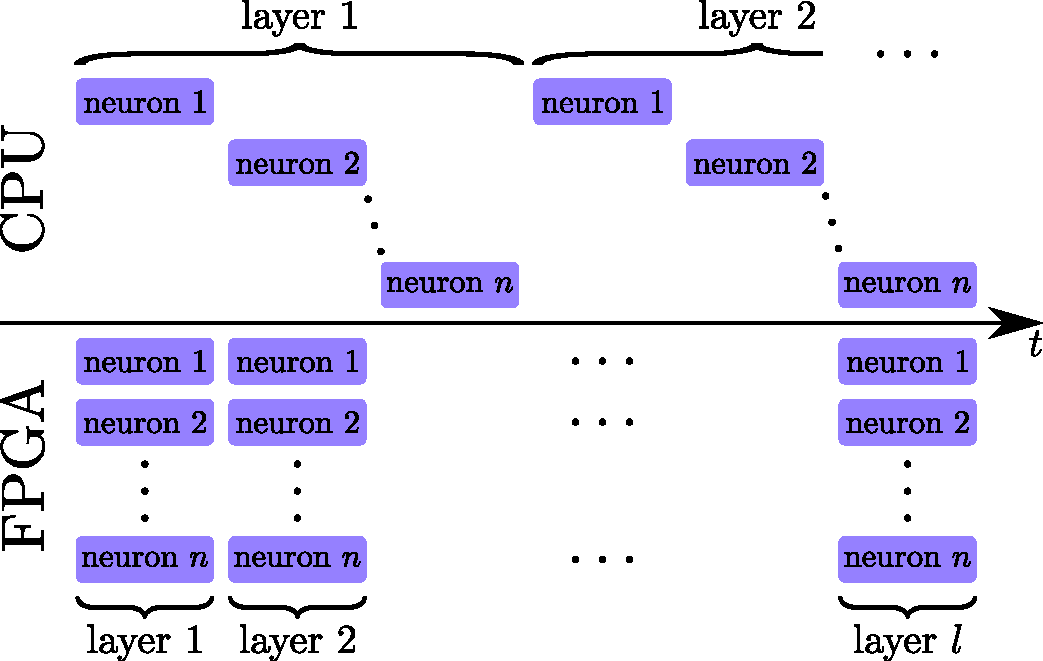
\includegraphics[scale=0.4]{fig/lec14/CPU_vs_FPGA.pdf}
	\caption{Conceptual comparison of CPU and FPGA evaluation of a neural network}
\end{figure}
\end{minipage}
\end{column}
\hfill
\begin{column}{0.45\textwidth}
\begin{minipage}[c]{\linewidth}
\begin{itemize}
	\item Each neuron has the same job $y_{n,l+1}=f(\bm{y}_{l}^\top\bm{w}_{n,l}+b_{n,l})$
	\item CPU must evaluate each neuron sequentially
	\item FPGA can evaluate each neuron at the same time
	\item Maximum number of parallel computations is limited
\end{itemize}
\end{minipage}
\end{column}
\end{columns}
}

%%%%%%%%%%%%%%%%%%%%%%%%%%%%%%%%%%%%%%%%%%%%%%%%%%%%%%%%%%%%%
%% Edge RL Pipeline %%
%%%%%%%%%%%%%%%%%%%%%%%%%%%%%%%%%%%%%%%%%%%%%%%%%%%%%%%%%%%%%
\frame{\frametitle{Edge reinforcement learning}
\begin{columns}[t,onlytextwidth]
\begin{column}{0.54\textwidth}
\begin{minipage}[c]{\linewidth}
	\vspace{0.25cm}
\begin{figure}
	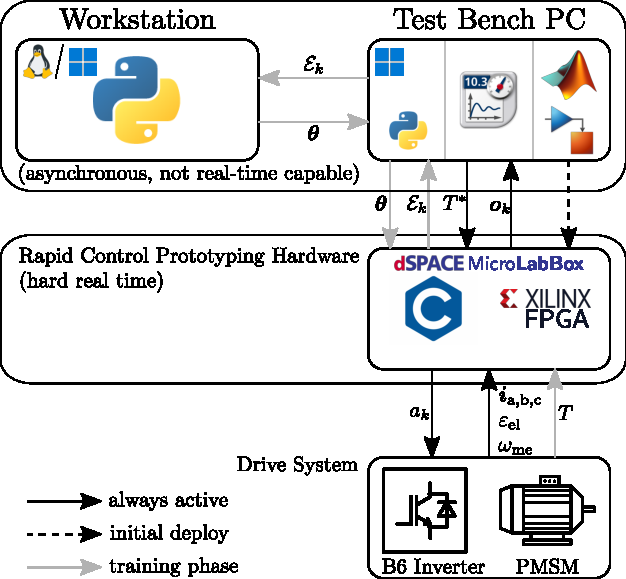
\includegraphics[scale=0.6]{fig/lec14/Edge_RL_Pipeline.pdf}
	\caption{Our edge reinforcement learning pipeline}
\end{figure}
\end{minipage}
\end{column}
\hfill
\begin{column}{0.45\textwidth}
\begin{minipage}[c]{\linewidth}
\begin{itemize}
	\item Backward pass / learning steps are outsource to workstation
	\item Communication between test bench and workstation is based on TCP/IP
	\item Backward pass is generic and has no time constraints $\rightarrow$ low application effort
\end{itemize}
\end{minipage}
\end{column}
\end{columns}
}

%%%%%%%%%%%%%%%%%%%%%%%%%%%%%%%%%%%%%%%%%%%%%%%%%%%%%%%%%%%%%
%% Demonstration video %%
%%%%%%%%%%%%%%%%%%%%%%%%%%%%%%%%%%%%%%%%%%%%%%%%%%%%%%%%%%%%%
\frame{\frametitle{Demonstration video}
\begin{tikzpicture}[overlay, remember picture]
	\node[anchor = center, inner sep=0pt, xshift=0.5cm] at (current page.center) {
		\href{https://www.youtube.com/watch?v=hQ49Mc6LV78&t=13}{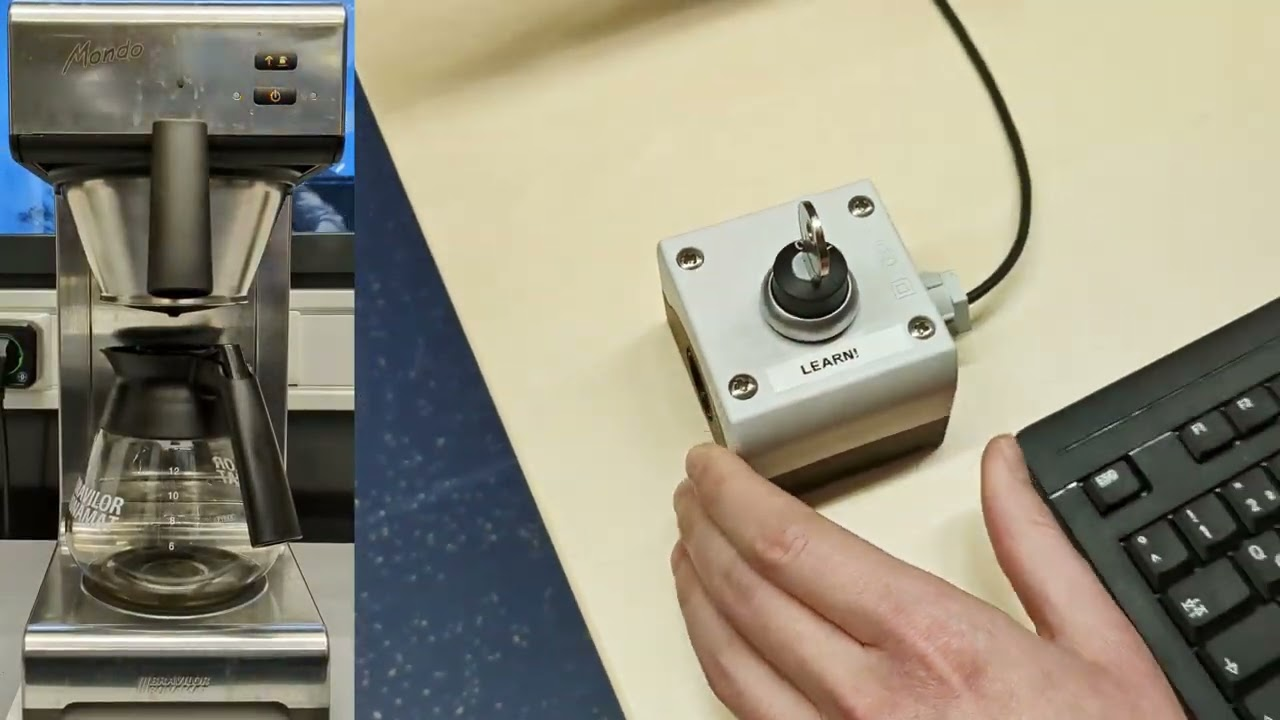
\includegraphics[width=0.7\paperwidth]{fig/lec14/Youtube_preview.jpg}}
	};
	\node[anchor = center, inner sep=0pt, xshift=0.5cm] at (current page.center) {
		\href{https://www.youtube.com/watch?v=hQ49Mc6LV78&t=13}{\fontsize{40}{60} \color{uniblue} \faYoutubePlay}
	};
\end{tikzpicture}
}
%%%%%%%%%%%%%%%%%%%%%%%%%%%%%%%%%%%%%%%%%%%%%%%%%%%%%%%%%%%%%%%%%%
\subsection{Meta reinforcement learning} 
%%%%%%%%%%%%%%%%%%%%%%%%%%%%%%%%%%%%%%%%%%%%%%%%%%%%%%%%%%%%%%%%%%

%%%%%%%%%%%%%%%%%%%%%%%%%%%%%%%%%%%%%%%%%%%%%%%%%%%%%%%%%%%%%
%% Problem setting %%
%%%%%%%%%%%%%%%%%%%%%%%%%%%%%%%%%%%%%%%%%%%%%%%%%%%%%%%%%%%%%
\frame{\frametitle{Meta reinforcement learning - the setting (1)}
\vspace{-0.1cm}
\begin{figure}%
\centering
\subfloat[][General problem class is similar, environments only differ in some characteristics, the agent could transfer learned behavior]{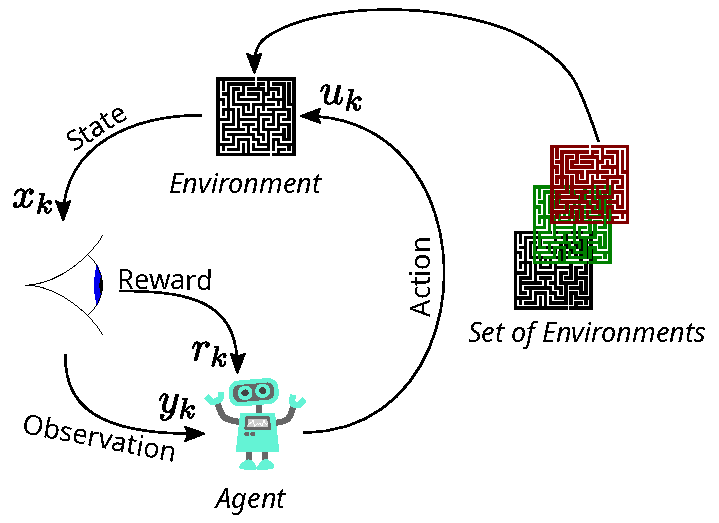
\includegraphics[scale=0.6]{fig/lec14/Meta_RL_Set_MDPS.pdf}}%
\qquad
\subfloat[][Solution approach: treat the environment as partially observable, distinguishing details are not directly available]{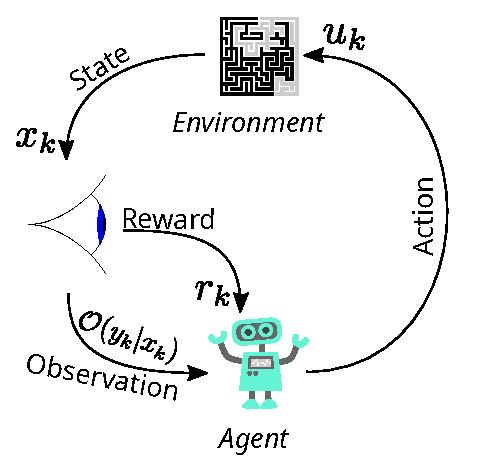
\includegraphics[scale=0.6]{fig/lec14/Meta_RL_POMDP.pdf}}%
\end{figure}
}

%%%%%%%%%%%%%%%%%%%%%%%%%%%%%%%%%%%%%%%%%%%%%%%%%%%%%%%%%%%%%
%% Problem setting %%
%%%%%%%%%%%%%%%%%%%%%%%%%%%%%%%%%%%%%%%%%%%%%%%%%%%%%%%%%%%%%
\frame{\frametitle{Meta reinforcement learning - the setting (2)}
\begin{columns}[t,onlytextwidth]
\begin{column}{0.45\textwidth}
\begin{minipage}[c]{\linewidth}
\begin{itemize}
	\item The agent must have some mechanism that allows adaptation to the specific environment
	\item This means, the distinguishing details must be extracted in some way
	\item Usually, they can be retrieved from a larger set of observations
\end{itemize}
\end{minipage}
\end{column}
\hfill
\begin{column}{0.54\textwidth}
\begin{minipage}[c]{\linewidth}
\begin{figure}
	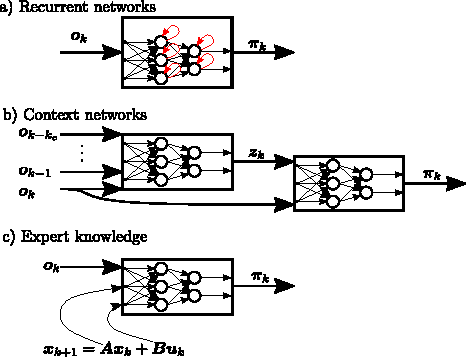
\includegraphics[scale=1.0]{fig/lec14/MetaLearningConcepts.pdf}
	\caption{Different concepts of meta learning}
\end{figure}
\end{minipage}
\end{column}
\end{columns}
}

%%%%%%%%%%%%%%%%%%%%%%%%%%%%%%%%%%%%%%%%%%%%%%%%%%%%%%%%%%%%%
%% Classical RL for drives %%
%%%%%%%%%%%%%%%%%%%%%%%%%%%%%%%%%%%%%%%%%%%%%%%%%%%%%%%%%%%%%
\frame{\frametitle{Usage in electric drive control: classical agent}
\begin{figure}
	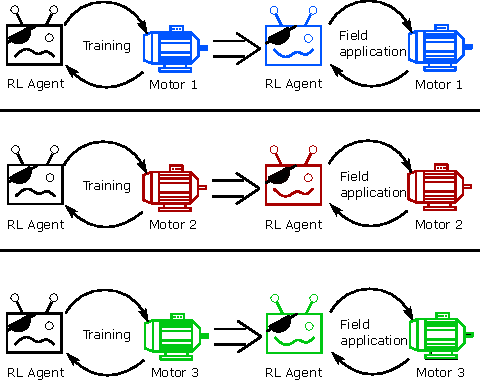
\includegraphics{fig/lec14/MetaProblemMotoren.pdf}
	\caption{Each agent must be trained individually $\rightarrow$ huge effort}
\end{figure}
}

%%%%%%%%%%%%%%%%%%%%%%%%%%%%%%%%%%%%%%%%%%%%%%%%%%%%%%%%%%%%%
%% Meta RL for drives %%
%%%%%%%%%%%%%%%%%%%%%%%%%%%%%%%%%%%%%%%%%%%%%%%%%%%%%%%%%%%%%
\frame{\frametitle{Usage in electric drive control: meta agent}
\begin{figure}
	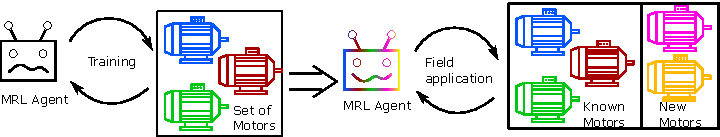
\includegraphics[scale=1.2]{fig/lec14/MetaLoesungMotoren.pdf}
	\caption{One agent to control them all $\rightarrow$ effort is limited and independent of the number of controlled environments}
\end{figure}
}

%%%%%%%%%%%%%%%%%%%%%%%%%%%%%%%%%%%%%%%%%%%%%%%%%%%%%%%%%%%%%
%% Proof of concept %%
%%%%%%%%%%%%%%%%%%%%%%%%%%%%%%%%%%%%%%%%%%%%%%%%%%%%%%%%%%%%%
\frame{\frametitle{Our setup}
\begin{columns}[t,onlytextwidth]
\begin{column}{0.4\textwidth}
\begin{minipage}[c]{\linewidth}
\begin{itemize}
	\item Make use of context network
	\item Generate context $\bm{z}$ with a fix set of observations $\rightarrow$ $\bm{z}=\text{const.}$
	\item Source: D. Jakobeit et al., \href{https://ieeexplore.ieee.org/abstract/document/10068250}{\textit{Meta-Reinforcement Learning-Based Current
Control of Permanent Magnet Synchronous Motor
Drives for a Wide Range of Power Classes}}, IEEE TPEL, 2023
\end{itemize}
\end{minipage}
\end{column}
\hfill
\begin{column}{0.65\textwidth}
\begin{minipage}[c]{\linewidth}
\begin{figure}
	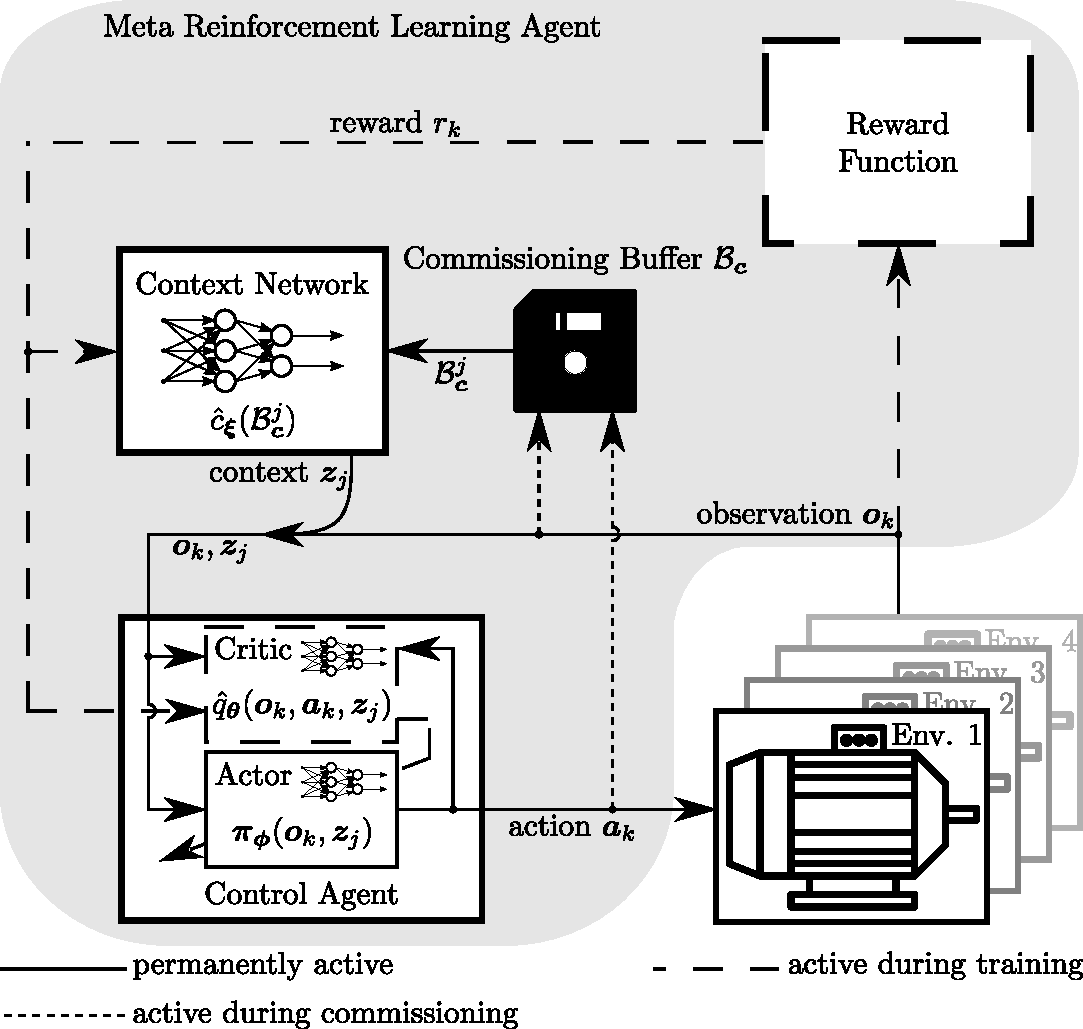
\includegraphics[scale=0.375]{fig/lec14/Meta_Scheme.pdf}
	\caption{A meta learning concept that we implemented successfully}
\end{figure}
\end{minipage}
\end{column}
\end{columns}
}

%%%%%%%%%%%%%%%%%%%%%%%%%%%%%%%%%%%%%%%%%%%%%%%%%%%%%%%%%%%%%
%% Evaluation %%
%%%%%%%%%%%%%%%%%%%%%%%%%%%%%%%%%%%%%%%%%%%%%%%%%%%%%%%%%%%%%
\frame{\frametitle{Evaluation on (very) different motors}
\vspace{-0.1cm}
\begin{figure}%
\centering
\subfloat[][Current control on a PMSM with low rated power]{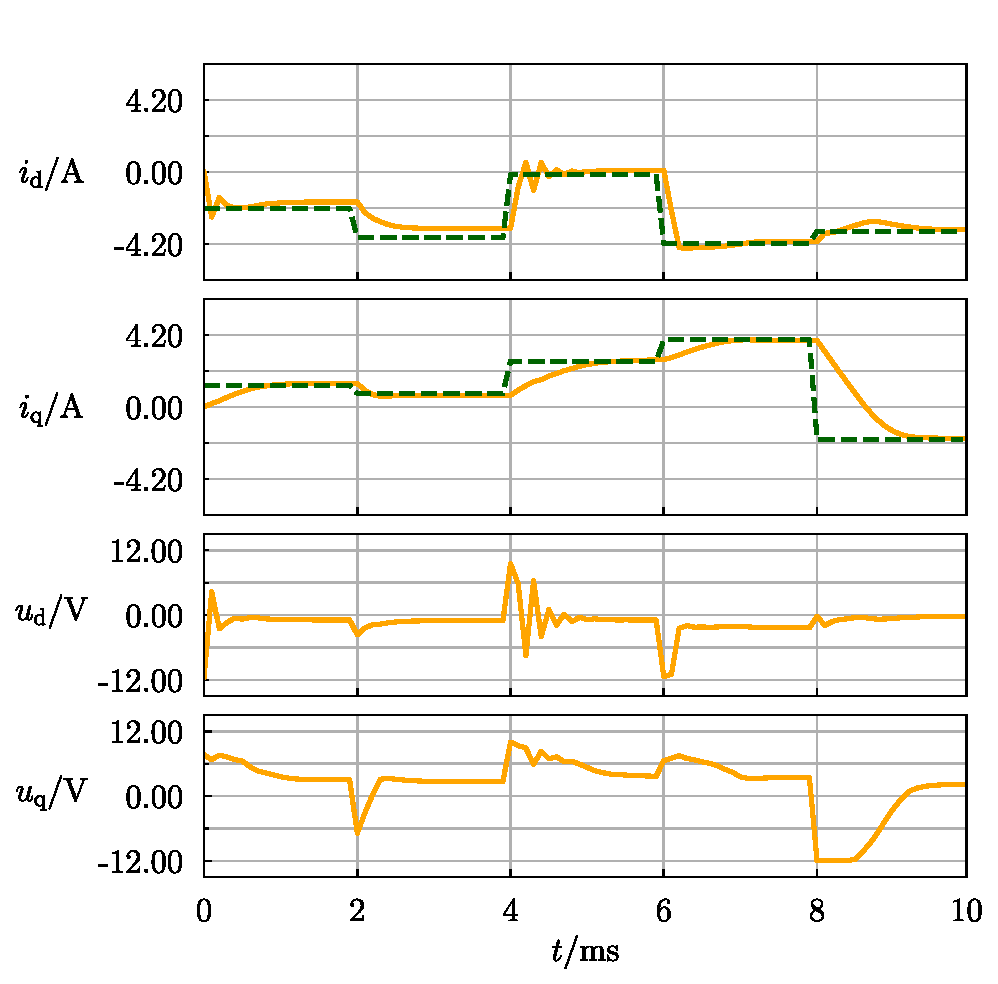
\includegraphics[scale=0.37]{fig/lec14/MetaLowPowerExample.pdf}}%
\qquad
\subfloat[][Current control on a PMSM with high rated power]{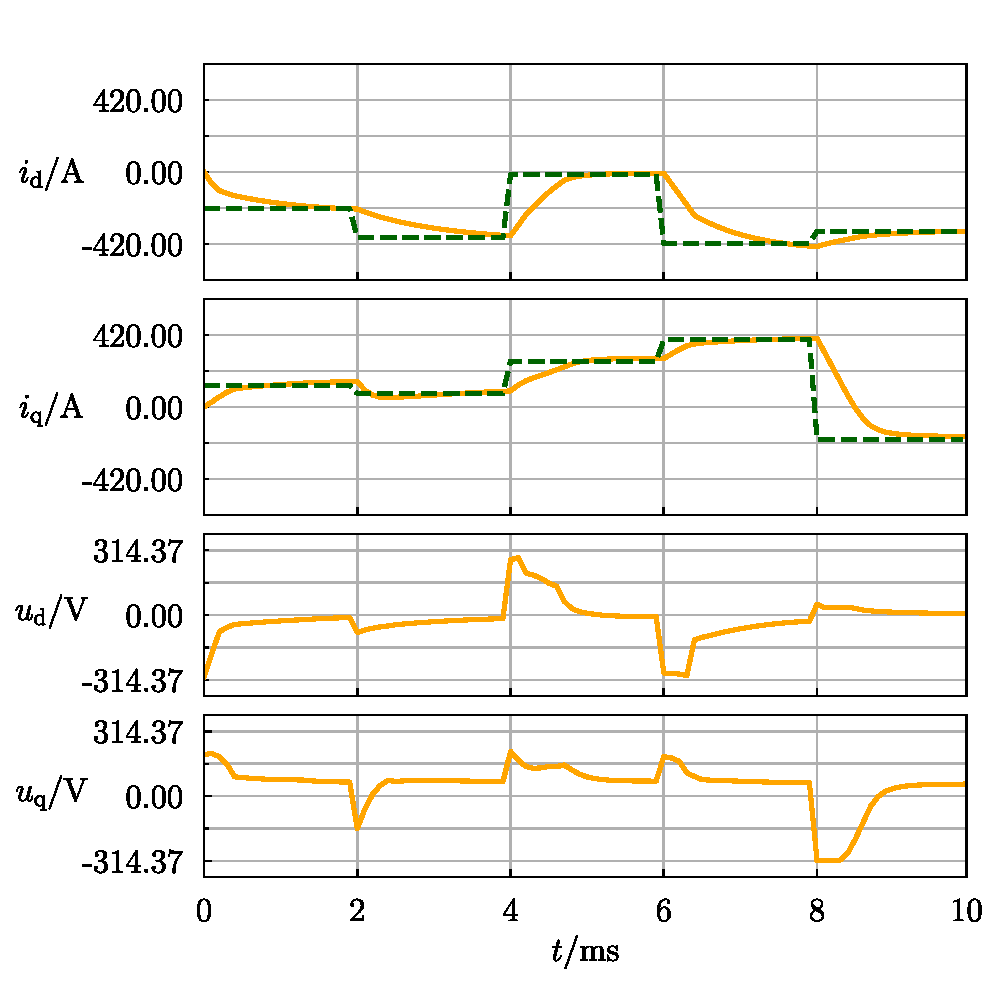
\includegraphics[scale=0.37]{fig/lec14/MetaHighPowerExample.pdf}}%
\end{figure}
}


%%%%%%%%%%%%%%%%%%%%%%%%%%%%%%%%%%%%%%%%%%%%%%%%%%%%%%%%%%%%%
%% Marketing %%
%%%%%%%%%%%%%%%%%%%%%%%%%%%%%%%%%%%%%%%%%%%%%%%%%%%%%%%%%%%%%
\frame{\frametitle{Summary}
\begin{itemize}
	\item Application of RL on technical systems comes with many challenges, e.g.,
	\begin{itemize}
		\item Safety limits,
		\item Real-time / computational constraints,
		\item Varying and/or partially unknown environments.
	\end{itemize}
	\item<2-> Real-world implementations often require more than bare RL algorithms, e.g.,
		\begin{itemize}
			\item<2-> Integration of available a priori expert knowledge,
			\item<2-> Combination with model-based control engineering tools.
		\end{itemize}
		\item<3-> Ideal integration of data-driven RL solutions together with expert-based control engineering parts is subject to many open research question. 
\end{itemize}
}
